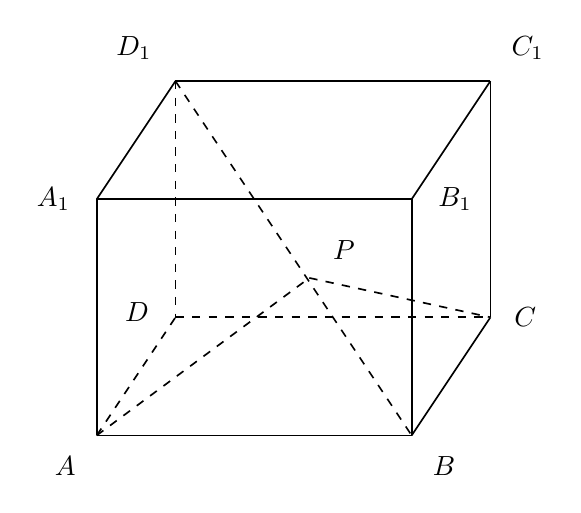
\begin{tikzpicture}[x=1cm,y=1cm,line width=.6pt,font=\normalsize]
\coordinate (A) at (0,0);
\coordinate (B) at (4,0);
\coordinate (C) at (5,1.5);
\coordinate (D) at (1,1.5);
\coordinate (Aone) at (0,3);
\coordinate (Bone) at (4,3);
\coordinate (Cone) at (5,4.5);
\coordinate (Done) at (1,4.5);
\coordinate (P) at (2.7,2.0);
% bottom/top solid
\draw (A) -- (B);
\draw (A) -- (Aone);
\draw (Aone) -- (Bone);
\draw (Bone) -- (B);
\draw (Aone) -- (Done);
\draw (Done) -- (Cone);
\draw (Cone) -- (Bone);
\draw (Cone) -- (C);
\draw (B) -- (C);
% hidden dashed cube edges
\draw[dashed] (A) -- (D);
\draw[dashed] (D) -- (C);
\draw[dashed] (Done) -- (D);
% diagonal and segments
\draw[dashed] (Done) -- (B);
\draw[dashed] (A) -- (P);
\draw[dashed] (P) -- (C);
% labels with clearance
\node[below left,xshift=-4pt,yshift=-4pt] at (A) {$A$};
\node[below right,xshift=4pt,yshift=-4pt] at (B) {$B$};
\node[right,xshift=5pt] at (C) {$C$};
\node[left,xshift=-6pt,yshift=2pt] at (D) {$D$};
\node[left,xshift=-6pt] at (Aone) {$A_{1}$};
\node[right,xshift=6pt] at (Bone) {$B_{1}$};
\node[above right,xshift=4pt,yshift=4pt] at (Cone) {$C_{1}$};
\node[above left,xshift=-5pt,yshift=4pt] at (Done) {$D_{1}$};
\node[above right,xshift=5pt,yshift=3pt] at (P) {$P$};
\end{tikzpicture}
